\documentclass{article}
\usepackage{amsmath}
\usepackage{amssymb}
\usepackage{graphicx}
\usepackage{hyperref}
\usepackage[version=4]{mhchem}

\title{Problem 1}
\date{}

\begin{document}
\maketitle

\section*{Problem}
A circle is inscribed in triangle \(A B C\). The tangent points are \(D, E, F\) as shown. Show that \(\angle F D E=90^{\circ}-\frac{1}{2} \angle A\).\\
\centering
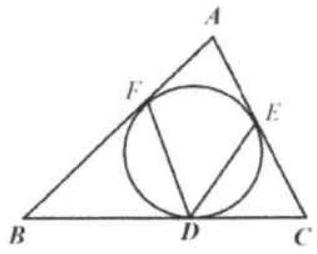
\includegraphics[width=\textwidth]{images/problem_image_1.jpg}

\section*{Solution}
Connect EF.\\
Since both \(A F\) and \(A E\) are tangent to circle \(O, A F=A E\) and \(\angle A F E=\angle A E F=\alpha\).\\
Thus \(\angle F D E=\alpha(\angle F D E, \angle A F E\), and \(\angle A E F\) face the same arc \(F E\) ).\\
In \(\triangle A E F, \angle A=180^{\circ}-2 \alpha \quad \Rightarrow \quad 2 \alpha=180^{\circ}-\angle A\)\\
That is \(\alpha=\angle F D E=90^{\circ}-\frac{1}{2} \angle A\).\\
\centering
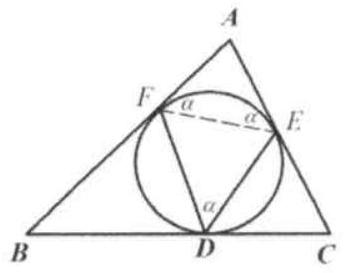
\includegraphics[width=\textwidth]{images/reasoning_image_1.jpg}

\end{document}
